\documentclass[conference]{IEEEtran}

\usepackage[british]{babel}
\usepackage{cite}
\usepackage{graphicx}
\usepackage{tabularx}
\usepackage[hyphens]{url}
\usepackage{amsthm}
\theoremstyle{definition}
\newtheorem{definition}{Definition}
\usepackage[textstyle,squaren]{SIunits}
\usepackage[pdftex,colorlinks=true]{hyperref}


% correct bad hyphenation here
%\hyphenation{op-tical net-works semi-conduc-tor}


\begin{document}
%
% paper title
\title{Measuring UK Crime Gangs}

% author names and affiliations
% use a multiple column layout for up to three different
% affiliations
\author{\IEEEauthorblockN{Giles Oatley}
\IEEEauthorblockA{Department of Computing\\
Cardiff Metropolitan University\\
Cardiff, UK\\
Email: goatley@cardiffmet.ac.uk}
\and
\IEEEauthorblockN{Tom Crick}
\IEEEauthorblockA{Department of Computing\\
Cardiff Metropolitan University\\
Cardiff, UK\\
Email: tcrick@cardiffmet.ac.uk}}

% conference papers do not typically use \thanks and this command
% is locked out in conference mode. If really needed, such as for
% the acknowledgment of grants, issue a \IEEEoverridecommandlockouts
% after \documentclass


% use for special paper notices
%\IEEEspecialpapernotice{(Invited Paper)}


% make the title area
\maketitle


\begin{abstract}
This paper describes the output of a study to tackle the problem of
gang-related crime in the UK; we present the intelligence and
routinely gathered data available to a UK regional police force, and
describe an initial social network analysis of gangs in the Greater
Manchester area of the UK between 2000-2006.

By applying social network analysis techniques, we attempt to detect
the birth of two new gangs based on local features (modularity,
cliques) and global features (clustering coefficient). Thus for the
future, identifying the changes in these can help us identify the
possible birth of new gangs (sub-networks) in the social system.

Furthermore, we study the dynamics of these networks globally and
locally, and have identified the global characteristics that tell us
that they are not random graphs -- they are small world graphs --
implying that the formation of gangs is not a random event. However,
we are not yet able to conclude anything significant about scale-free
characteristics due to insufficient sample size.
\end{abstract}

% For peer review papers, you can put extra information on the cover
% page as needed:
% \ifCLASSOPTIONpeerreview
% \begin{center} \bfseries EDICS Category: 3-BBND \end{center}
% \fi
%
% For peerreview papers, this IEEEtran command inserts a page break and
% creates the second title. It will be ignored for other modes.
\IEEEpeerreviewmaketitle


\section{Introduction}\label{sec:introduction}

There have been numerous studies of criminal networks and gangs; as
highlighted in \cite{hughes:2005}, the popularity of qualitative
studies of gang-related issues soared during the 1980s and 1990s,
following renewed media and public interest, statistical advances, and
increased government funding. Qualitative studies have taken three
major forms: (a) surveys of law enforcement officials (and at times
other agency personnel) regarding gangs in their jurisdictions and
actions taken to control them, (b) analyses of data compiled by law
enforcement agencies and/or court officials, and (c) self-reports of
samples of youth and/or young adults.  There have been calls for
research evidence to be drawn into police practice, but development of
such an agenda has been hampered by a range of
factors~\cite{bullock+tilley:2009}. Research into youth gangs,
especially the age at which youths join gangs and the early
precursors, has been conducted in the USA and Canada
\cite{hill-et-al:2001}, China \cite{webb-et-al:2011} and Hong Kong
\cite{lo:2011}.

However, the UK has been slow in carrying out research into gang crime
(excepting work done in North East London~\cite{pitts:2007} in 2007),
and especially into what actions work best at controlling it. In
Greater Manchester, a region in the north of the UK that has had a
significant gun crime problem related to gang activity (primarily due
to acute social deprivation in the
area)~\cite{BBCNews2003,BBCNews2004,HalesLewisSilverstone2006}, recent
police initiatives have started to address this problem
\cite{BBCNews2010}.

Social network analysis has been applied across a wide number of
domains, providing a unifying language to describe disparate systems
ranging from social interactions to power grids. There is also a
growing body of literature applied to crime analysis (for example:
\cite{BaronTindall1993,Klerks2001,Hansen2005,OatleyZeleznikowLearyEwart2005,OatleyEwartZeleznikow2006,CalvoArmengolZenou2006,HutchinsBenhamHutchins2009}).
Related work~\cite{CalvoArmengolVerdierZenou2007,PatacchiniZenou2008}
on analysing the strength of weak ties in crime through steady state
equilibria modelling has also been successful. Identifying structural
holes, betweenness and social capital reinforces the value of using
social network analysis for gang research~\cite{papachristos:2006}.

We present the dynamics of a social network study of these gangs and
their associates, using the intelligence gathered by police
observations of known gang members and associated criminals. We
develop the statistical analysis of network dynamics, combining
well-known global topological measures, local motifs and
modules~\cite{CostaRodriguesTraviesoVillasBoas2007,Jackson2008,Newman2003}.
Network motifs are subgraphs that appear more frequently in a real
network than could be statistically expected. At a global level, if
these networks of associations exhibit clustering behaviour this
indicates the presence of gangs. At a local level, any defined
substructures will provide us information about the gang structure. We
are interested in modelling the dynamics of the gangs, their
development and fragmentation into new gangs, and we hope that the
study of the dynamics in such modules will provide information on the
structural changes within gangs that lead to birth of new gangs, and
predictors of other gang-related behaviour.

Furthermore, we investigate if the networks have scale-free,
small-world or other characteristics
\cite{Watts1999,AlbertBarabasi2002,Newman2003}; small-world networks
are characterised by a diameter that grows logarithmically with their
size. One important characteristic of the small-world phenomenon is
that each pair of nodes are connected through a relatively small
number of steps to a huge network size defined by the total number of
nodes. Scale-free structures consists of many nodes with low degrees
and a few hubs with high
degrees~\cite{AlbAlbNak04,CostaRodriguesTraviesoVillasBoas2007,Jackson2008}. If
the offender networks can be classified into either (or both) of these
categories (or other known network types), then this provides not only
insight into the dynamics of the gang network, but also operational
uses; for instance, network disruption/destruction strategies,
nodes/offenders to monitor, and so on.


\section{Problem description and data}\label{sec:problemdescription}

Gun crime in Manchester first gained media attention in 1988 after
concern over eight shootings and a gun-related murder, at a time when
gun crime was considered rare in the UK. Nevertheless, gun crime in
Manchester appears to have begun in the late 1970s at a time of rising
unemployment and poverty in the area.

Numerous shootings -- both fatal and non-fatal -- have taken place
over the years as the the Pepperhill, Gooch, Doddington and Longsight
Crew gangs (see Table~\ref{table:gangnames}) have clashed over drug
territories and other disputes. Many of these gun fire exchanges were
on public streets, some were planned acts and some were spontaneous
events.

\begin{table}[htb]
\centering
\begin{tabularx}{\columnwidth}{c X c}
%\begin{tabular}{c c c} 
\hline
Gang label & Gang Name & Formation  \\ %[0.5ex]
\hline
A & Gooch & 1990s\\
B & Doddington/Pepperhill & 1990s\\
C & Longsight Crew &  c.2001\\
D & Rusholme Crew Gangsters & c.2004\\ %[1ex] % [1ex] adds vertical space 
\hline
%\end{tabular}
\end{tabularx}
\caption{Gang names and approximate dates of formation.}
\label{table:gangnames}
\end{table}

In 2001, a new approach to tackling gun crime began to develop with
police working more closely with the local community and other
agencies. The Manchester Multi-Agency Gang Strategy (MMAGS), a
multi-agency approach to tackling gun crime and detering young people
from entering into a gang/gun culture was initiated as a result of a
UK Home Office report~\cite{BullockTilley2002}. The report concludes
that about 60 per cent of shootings are thought to gang-related, with
violence in general, and gun violence and fatal shootings inparticular
are concentrated in specific small areas of South Manchester, and that
gangs in South Manchester are loosely turf-based.

The geographical proximity of the gang locations and hub of all these
activities can be seen in Figure \ref{fig:serious}, where the distance
between Gangs A and B is hundreds of meters, literally a few streets
away from each other.  Gangs A and B show a negative attitude towards
each other, often resulting in `tit-for-tat' gun crimes. The alignment
between Gangs A and D is possibly because of a mutual rivalry with B,
while the positive alignment of B with C is because A has encroached
on C's `territory' for drug sales. The gang locations are overlaid on
the locations of all serious crimes (murder, attempted murder,
manslaughter, kidnapping, serious wounding, and firearms offences)
recorded in the data available to the consortium for the period
1980-2007. Agreeing strongly with the Home Office
report~\cite{BullockTilley2002} we find: 38\% (n=162) of all serious
crimes occurring within \unit{1}{\kilo\meter} radius (of gang
locations) and 63\% of all serious crimes occur within
\unit{2}{\kilo\meter}, and 53\% (n=9) of murders are within
\unit{3}{\kilo\meter}; 38\% (n=34) of attempted murders are within
\unit{1}{\kilo\meter} and 63\% within \unit{2}{\kilo\meter}; and, 33\%
(n=17) of serious woundings are within \unit{1}{\kilo\meter} and 48\%
are within \unit{2}{\kilo\meter}.

\begin{figure}[!ht] 
\centering
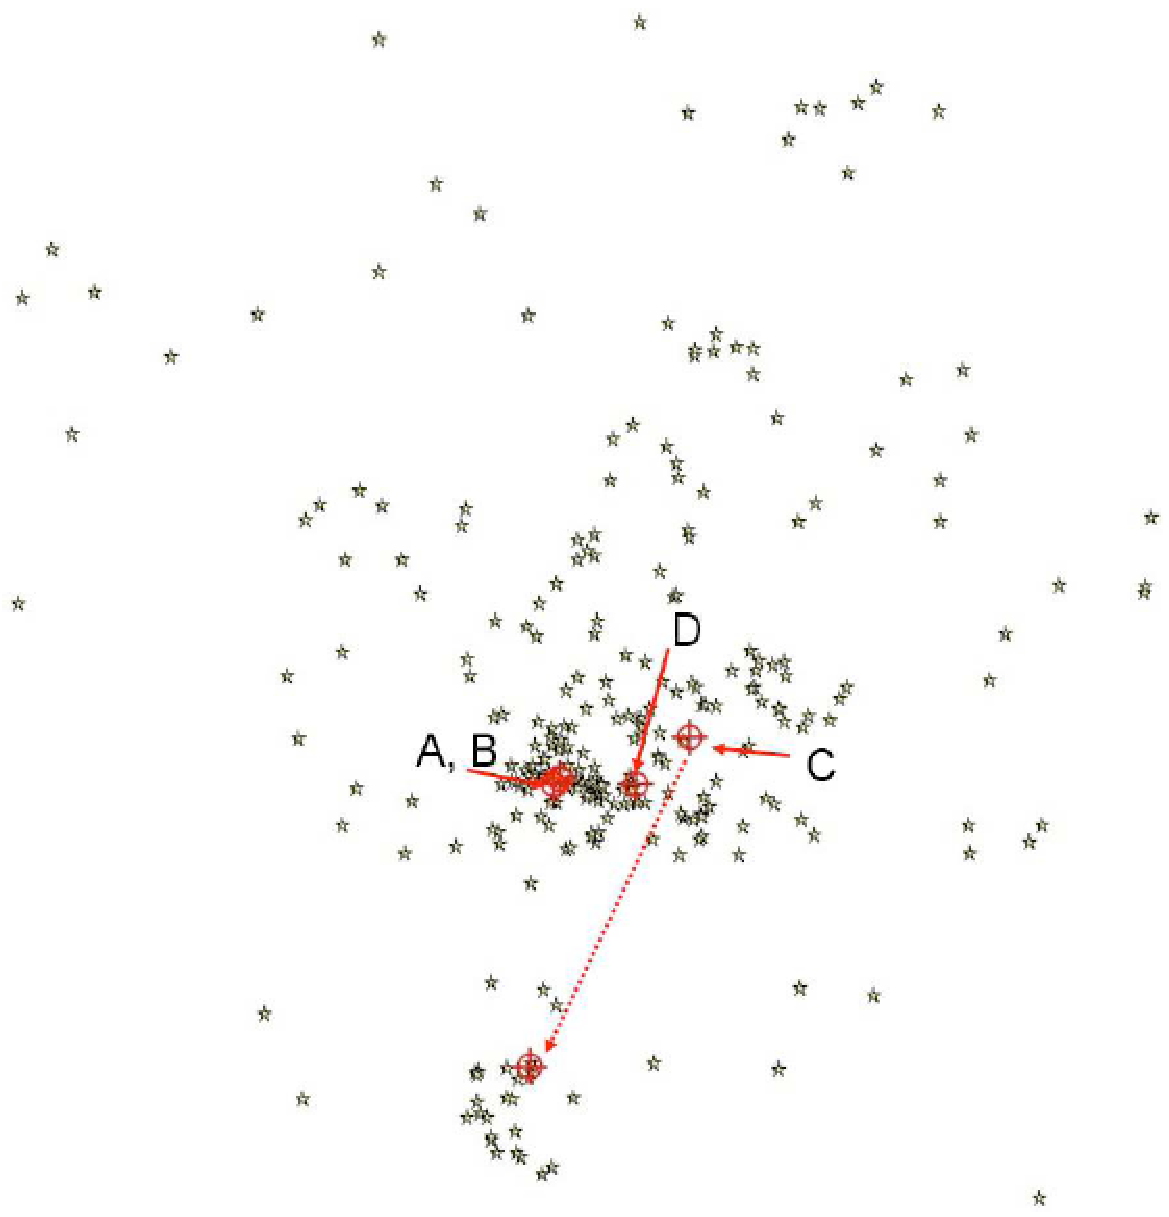
\includegraphics[width=\columnwidth]{images/serious}
\caption{All serious crimes: murder, attempted murder, manslaughter,
kidnapping, serious wounding, firearms offences. Gang C has moved into
an additional location with drug selling. Gang geographical locations. \emph{positive} indicates a positive alignment between the gangs, \emph{negative} indicates negative alignment.}
\label{fig:serious}
\end{figure}


\section{Police databases}\label{sec:policedatabases}

The database used for this analysis included the list of associates
for each gang member, with fields such as unique identifiers for each
offender, date of birth, relationship between the offenders, ethnic
origin, reason reported and date of occurrence.


\subsection{Link types}\label{sec:linktypes}
The network links available are quite different to other existing work
with networks of burglars or retail fraudsters
\cite{OatleyZeleznikowLearyEwart2005,OatleyMcGarryEwart2006}). Examples
of the data (link types) from which the networks of offenders
are developed can be found in Table~\ref{tab:associates}. These link
types are: \emph{Accomplice}; \emph{Brother-Brother};
\emph{Boyfriend}; \emph{Brother}; \emph{Sister}; \emph{Charged with};
\emph{Child}; \emph{Cohabitant}; \emph{Foster child}; \emph{Foster
parent}; \emph{Friend}; \emph{Girlfriend}; \emph{Guardian};
\emph{Other}; \emph{Parent}; \emph{Relative}; \emph{Spouse};
\emph{Sister-Sister}; \emph{Ward}; \emph{Gay Boyfriend}; and \emph{Gay
Girlfriend}.

An explanation of the dataset from Table~\ref{tab:associates} follows,
and it is clear that it is a rich source of information. However,
there are also many inconsistencies, and if this data is to be used to
its full potential it will require a great deal of pre-processing,
using natural language processing, matching with regular expressions,
information extraction, and so on. There should also be further
categorisation applied, considering that 50\% of the data is
classified of type \emph{Other}.


\begin{table*}[!ht]
\resizebox{\textwidth}{!}{
\begin{tabular}{|c|l|l|l|}
\hline
\multicolumn{1}{|l|}{Magnet Category} & Relationship & Frequency/Percentage & Reason Reported Examples \\ 
\hline
\multicolumn{1}{|l|}{Crime related} & 1.\ Accomplice & 502, 10.7\% & (i.) Arrested Together \\ 
  &   &   &  (ii.) Believed To Be Dealing Drugs Together \\ 
  &   &   &  (iii.) X's Sister Is Y's Girlfriend \\ \cline{2-4}
  &  2.\ Charged with &  45, 1.0\% &  (i.) Charged Together Murder \\ 
  &   &   &  (ii.) Arrested Together \\ 
\hline
\multicolumn{1}{|l|}{Familial} &  3.\ Brother &  65, 1.4\% &  (i.) Believed To Be Half-Brothers \\ \cline{2-4}
  &  4.\ Child &  23, 0.5\% &  (i.) Father \& Son \\ 
  &   &   &  (ii.) Admitted Above Named Is His Dad \\ \cline{2-4}
  &  5.\ Parent &  20, 0.4\% &  (i.) Mother \& Son \\ \cline{2-4}
  &  6.\ Relative &  173, 3.7\% &  (i.) Cousins \\ 
  &   &   &  (ii.) X States Y Is His Uncle \\ \cline{2-4}
  &  7.\ Sister &  18, 0.4\% &  (i.) Brother And Sister \\ 
  &   &   &  (ii.) Stated They Are Brothers \\ \cline{2-4}
  &  8.\ Spouse &  2, 0.0\% &  (i.) Arrested Together Handling \\ 
\hline
\multicolumn{1}{|l|}{Friendships} &  9.\ Cohabitant &  5, 0.1\% &  (i.) Possibly Living Together At Anon Street \\ \cline{2-4}
  &  10.\ Friend &  1409, 30.0\% &  (i.) Stop Checked Together In car \\ 
  &   &   &  (ii.) Attended Club Together \\ 
  &   &   &  (iii.) Seen Together \\ \cline{2-4}
  &  11.\ Girlfriend &  61, 1.3\% &  (i.) Have Child Together \\ \cline{2-4}
  &  12.\ Boyfriend &  10, 0.2\% &  (i.) Girlfriend/Boyfriend \\ 
\hline
\multicolumn{1}{|l|}{Other} &  13.\ Other &  2364, 50.3\% &  (i.) Ex-Boyfriend Of The Above Named \\ 
  &   &   &  (ii.) R Claimed E Stabbed Him \\ 
  &   &   &  (iii.) C Intends Killing A/N Re Murder Of Bros \\ 
  &   &   &  (iv.) Tog At Nightclub, Oldham \\ 
  &   &   &  (v.) Seen Together \\ 
  &   &   &  (vi.) Attended Murder Trial \\ 
  &   &   &  (vii.) Arrested Together In Anon \\ 
  &   &   &  (viii.) D's Number In C's Mobile \\ 
  &   &   &  (ix.) Seen Together At Moss Side Festival \\ 
\hline
\end{tabular}}
  \caption{Examples of the `associates' data. This data is used to
    create the social networks. Gang membership comprises a mix of same-age local friendship
groups, blood relatives and recruits: UK Home Office
report~\cite{BullockTilley2002}.}
  \label{tab:associates}
\end{table*}


\subsection{Observations and inconsistencies in the dataset}\label{sec:observations}
The following indices refer to rows in Table~\ref{tab:associates}, for
instance \emph{1-i} refers to \emph{1. Accomplice} from the
\emph{Relationship} column, and \emph{(i.) Arrested Together} from
the \emph{Reason Reported Examples} column.

\begin{itemize}
\item	\emph{1-i} and \emph{2-ii} indicate that the data is not rigidly recorded or categorised 
\item	\emph{1-iii} is incorrectly categorised
\item	\emph{3-i}, \emph{6-ii} and \emph{9-i} illustrate that the
  intelligence is fallible, and is often based upon beliefs, and also
  that the link types are not all of equivalent strength, for instance
  the strength of a \emph{Belief} link (possibly false) versus a \emph{Charged
  Together} link (definitely true)
\item	\emph{4-i} and \emph{5-i} illustrate how the same information can be described, often in different forms, in separate fields
\item	\emph{7-ii} shows an obvious mistake with \emph{Brothers} recorded in the \emph{Sisters} category
\item	\emph{8-i} contains not only information about cohabitation, but also intelligence about handling stolen goods
\item	\emph{11-i} illustrates again that links can be stronger or weaker, for instance the child may mean that there is a stronger bond/link between the offenders
\item	\emph{10-i-iii} could all be placed in the \emph{Other} category
\item	\emph{13-ii,iii} contain a lot of intelligence
\item	\emph{13-v} is a weak form of link, and should really indicate whether it was on good or bad terms
\item	\emph{13-vii} should be in either the \emph{Accomplice} or
  \emph{Charged With} categories
\item	\emph{13-viii} is noteworthy as it is a very specific link, a mobile phone link
\end{itemize}


\subsection{Limitations of the data and affects to SNA}\label{sec:limitations}
Overall, it is concerning that this data is used as a gang database, but
without explicit qualifications. Furthermore, it is generally not
purged, but membership would not necessarily have an effect on
sentencing.  Comparing to gang criteria by states in the USA,
`{\emph{Identified by reliable source (police)}}', and
`{\emph{associates with members}}' would secure membership in Florida
\cite{barrows-huff:2009}.


Criticism of gang databases ranges from the position of being
`unconstitutional' if they are not correctly maintained, for instance,
not regularly purged of citizens who have left the gang world
\cite{jacobs:2009}, to including inaccuracies:

\begin{quote}
``{\emph{In sum, gang databases appear to be riddled
with factual inaccuracies, administrative errors, lack of compliance
with departmental guidelines, and lack of oversight. But this is not
the worst of it. The root of the problem may be that even if properly
applied, application of the subjective criteria would not produce
useful results.}}''~\cite{wright:2005}
\end{quote}


It is important to be critical of information about gangs that come
from the police or from journalists, which is often based on
impressions and not on thorough research. For instance 'intelligence'
that describes that there are leaders in gangs who are responsible for
'recruitment' is at odds with our findings, that our network data does
not find any obvious leadership (which is in line with many
criminological studies on gangs). Various network outcomes contradict
current stereotypes of gang behavior, for example the existence of
many links and intermediaries between different and sometimes
conflicting gangs.


\section{Identifying community structure}\label{sec:communitystructure}
In order to investigate community structure we removed any nodes with
less than six connections (i.e. degree 6);
Figure~\ref{fig:2002core_labelled} shows data from 2002, with the
well-established Gangs A and B, and also the newly formed Gang C (in
2001). The Gangs A, B, and C are highly interconnected, with
Figure~\ref{fig:2002core_labelled} also showing the `go-betweens',
labelled as \emph{ab*} and \emph{bc*}. Individuals who are only
connected to one gang, and who are highly connected within themselves,
are labelled \emph{a*} and \emph{b*}. In this way it is easier to see
the communities.


\begin{figure}[htb]
\centering
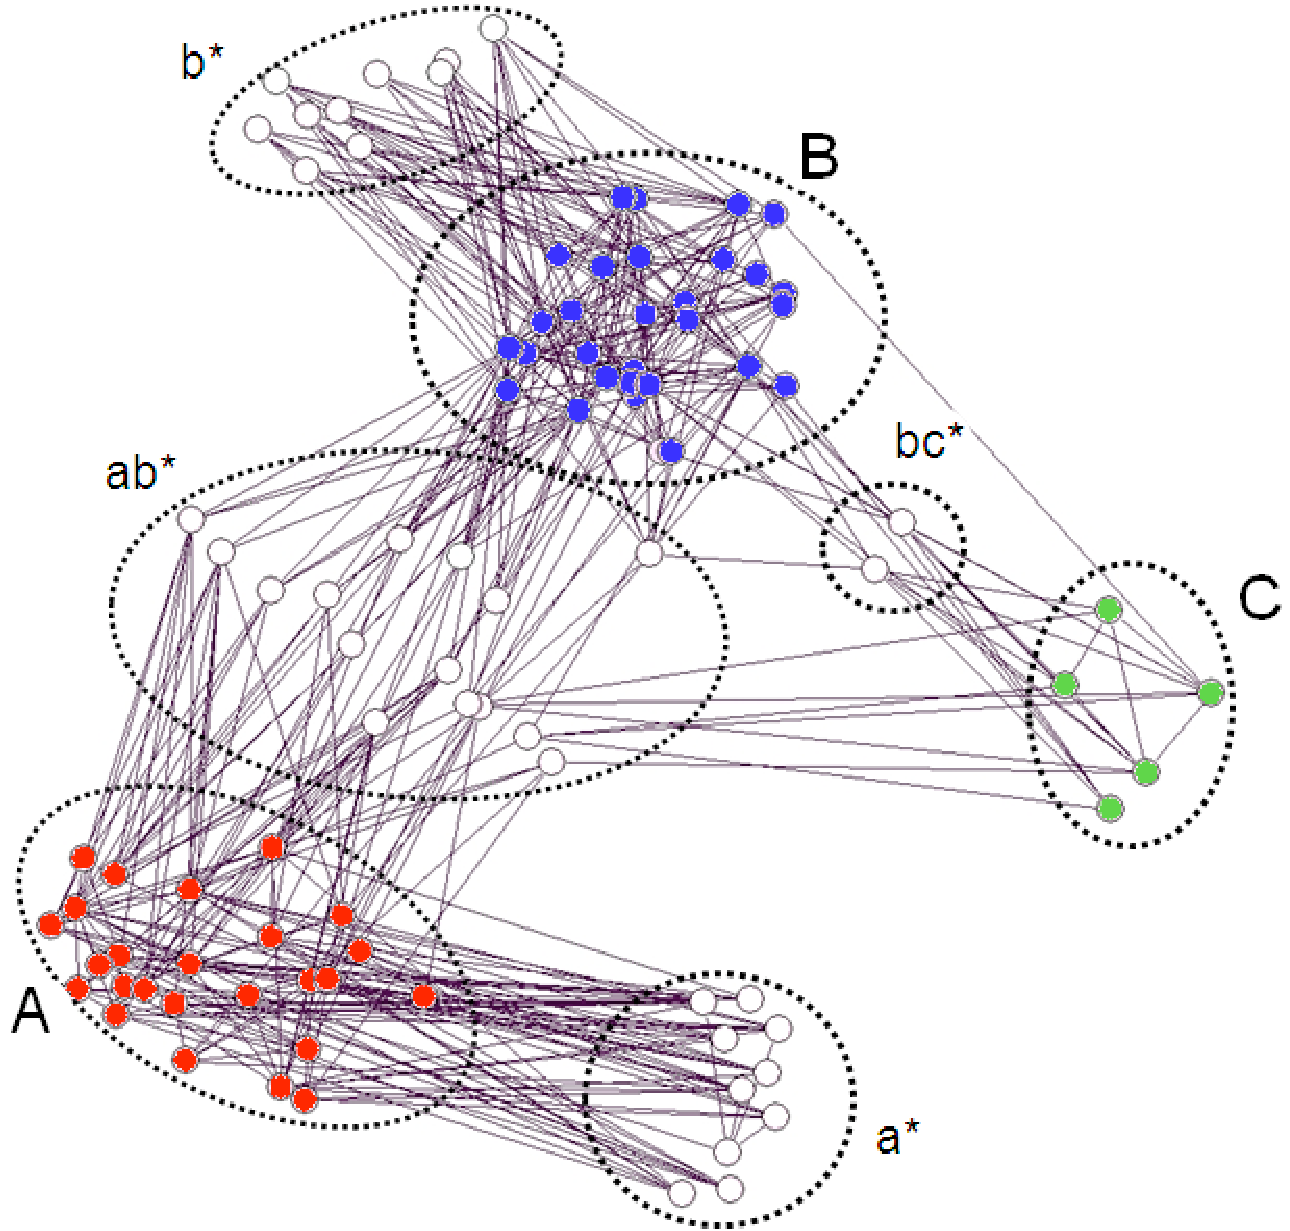
\includegraphics[width=\columnwidth]{images/2002core_labelled}
\caption{Link reduction, showing Gangs A and B and emergence of
  Gang C (for 2002). This also illustrates the large amount of non-gang
  members who are associated with individual gangs (\emph{a*}, \emph{b*}) or who are intermediaries (\emph{ab*}, \emph{bc*}).}
\label{fig:2002core_labelled}
\end{figure}


\section{Network characterisation}\label{sec:networkcharacteristics}
A series of experiments were carried out to determine how the gang
networks compare with well-known networks, for example scale-free and
small-world networks.

\subsection{Small-world networks}\label{sec:smallworld}
Table~\ref{tab:networkmeasuresyears} presents the clustering
coefficient~\cite{WattsStrogatz1998} (CC) for each individual year,
alongside the node and edge counts and various other measures to
describe the network. For any simple connected graph \emph{G} with at
least two vertices, the clustering coefficient (1-neighbourhood)
\cite{WattsStrogatz1998} measures the extent to which vertices linked
to any given vertex \emph{v} are also linked to each other. Or in
other words, are the friends of my friends also my friends? This is
1-neighbourhood clustering. The clustering coefficient 2-neighbourhood
is a less stringent condition, and states: of the friends of my
friends, are they linked to me by other friends?

The links presented in Table~\ref{tab:networkmeasuresyears} are
cumulative; that is, the links and nodes for 2002 include not only the
new links and nodes for 2002, but also those for 2001 and 2000.

\begin{table}[htb]
\resizebox{\columnwidth}{!}{
\begin{tabular}{|l|r|r|r|r|r|r|r|}
\hline
 Measure &  2000 &  2001 &  2002 &  2003 &  2004 &  2005 &  2006 \\ 
\hline
 Number of nodes (n) &  1095 &  1295 &  1487 &  1752 &  2090 &  2229 &  2408 \\ 
\hline
 1/n &  0.00091 &  0.00077 &  0.00067 &  0.00057 &  0.00048 &  0.00045 &  0.00042 \\ 
\hline
 4/n &  0.00365 &  0.00309 &  0.00269 &  0.00228 &  0.00191 &  0.00180 &  0.00166 \\
\hline
 log(n) &  6.999 &  7.166 &  7.305 &  7.469 &  7.645 &  7.709 &  7.787 \\ 
\hline
 log(log(n)) &  1.95 &  1.97 &  1.99 &  2.01 &  2.03 &  2.04 &  2.05 \\ 
\hline
 Number of links &  1565 &  1903 &  2295 &  2844 &  3540 &  3872 &  4265 \\ 
\hline
 Total possible links &  598965 &  837865 &  1104841 &  1533876 &  2183005 &  2483106 &  2898028 \\ 
\hline
 Diameter &  12 &  14 &  11 &  11 &  14 &  12 &  13 \\
\hline
 Average path length &  4.85 &  4.82 &  4.68 &  4.57 &  4.86 &  4.78 &  4.70 \\ 
\hline
 Density &  0.00261 &  0.00227 &  0.00208 &  0.00185 &  0.00162 &  0.00156 &  0.00147 \\ 
\hline
 Betweenness &  0.107 &  0.117 &  0.172 &  0.205 &  0.146 &  0.102 &  0.100 \\ 
\hline
 CC (cumulative) &  0.47 &  0.48 &  0.47 &  0.46 &  0.49 &  0.55 &  0.56 \\ 
\hline
 CC (per year) &  0.24 &  0.57 &  0.34 &  0.15 &  0.62 &  0.25 &  0.30 \\ 
\hline
\end{tabular}}
\caption{Network measures for 2000-2006. Clustering coefficients are always greater than 4/n. Average path lengths are always less than log(n).}
\label{tab:networkmeasuresyears}
\end{table}


Table~\ref{tab:networkmeasuresgang} shows the same network measures,
but this time the data has been sliced into the members of the Gangs
A, B, C and D.


\begin{table}[htb]
\resizebox{\columnwidth}{!}{
\begin{tabular}{|l|r|r|r|r|}
\hline
 Measure & \multicolumn{1}{c|}{A} & \multicolumn{1}{c|}{B} & \multicolumn{1}{c|}{C} & \multicolumn{1}{c|}{D} \\
\hline 
 Number of nodes (n) &  859 &  617 &  431 &  513 \\ 
\hline
 1/n &  0.00116 &  0.00162 &  0.00232 &  0.00195 \\ 
\hline
 4/n &  0.00466 &  0.00648 &  0.00928 &  0.00780 \\ 
\hline
 log(n) &  6.76 &  6.42 &  6.07 &  6.24 \\ 
\hline
 log(log(n)) &  1.91 &  1.86 &  1.80 &  1.83 \\ 
\hline
 Number of links &  844 &  1047 &  602 &  707 \\ 
\hline
 Total possible links &  368511 &  190036 &  92665 &  249571 \\ 
\hline
 Diameter &  7 &  5 &  6 &  7 \\ 
\hline
 Average path length &  3.61 &  3.38 &  3.37 &  4.11 \\ 
\hline
 Density &  0.00396 &  0.00550 &  0.00648 &  0.00537 \\ 
\hline
 Closeness &  0.302 &  0.298 &  0.393 &  0.305 \\ 
\hline
 Betweenness &  0.185 &  0.179 &  0.350 &  0.239 \\ 
\hline
 CC &  0.16 &  0.19 &  0.15 &  0.12 \\ 
\hline
\end{tabular}}
\caption{Network measures for Gangs A, B, C, D. CC is the  average clustering coefficient from~\cite{WattsStrogatz1998}, considering only 1-neighbourhood.}
\label{tab:networkmeasuresgang}
\end{table}

A small-world network has both local connectivity and global
reach~\cite{WattsStrogatz1998}, and is a simple connected graph
\emph{G} exhibiting two properties:

\begin{enumerate}
\item Small characteristic path length: the presence of short-cut
connections between some vertices results in a small characteristic
path length \emph{L(G)}.
\item Large clustering coefficient: each vertex of \emph{G} is linked
to a relatively well-connected set of neighbouring vertices, resulting
in a large value for the clustering coefficient \emph{C(G)}.
\end{enumerate}
 
To determine whether our network is a random one or is small-world, we
can test whether or not it has exponential \emph{k}-connectivity
distribution. We do not observe this in the data, however, we do see
large clustering coefficients, and the average path lengths are always
less than {\emph{log(n)}}. Based upon these two criteria we can still
conclude that our networks have small-world characteristics.


\subsection{Scale-free networks}\label{sec:scalefree}
This section also refers to the preceding tables, where we find a
mixture of evidence for and against the case for scale-free networks.

Plotting the clustering coefficient as a function of the number of
nodes $n$, should follow the power-law distribution for scale-free
networks (see later experiments), with the clustering coefficient
being roughly four times larger than random networks
\cite{AlbAlbNak04}. The value of the clustering coefficient for a
random networks will be \emph{1/n}. In this way we are able to compare
the values of \emph{4/n} against CC in
Tables~\ref{tab:networkmeasuresyears} and
\ref{tab:networkmeasuresgang}. As the cumulative links increase from
2000 to 2006, the value of CC generally increases (with the number of
nodes n) and is always significantly higher than the values of
\emph{4/n}. Each of the gang values for CC are also significantly
higher than would be expected in a random network.

The diameter of the network (longest path length) should be
approximately \emph{log(log(n))} for scale-free networks. In both
cases (for the gangs and the years) the real values are significantly
higher than would be expected for a scale-free network.

The average path length should be approximately \emph{log(n)} for
scale-free networks. For both the `years' and `gangs' data it was
actually smaller than \emph{log(n)}, indicating scale-free networks.

The statistics on degree centrality were low, indicating that there is
no group leader. As we know when Gangs C and D are formed (2001
and 2004 respectively), it is interesting to note that the
characteristic of the networks at this time are that the betweeness
centralisation reaches 0.2. It is necessary to compare the closeness and
betweenness averages for each gang against the value for the overall
network.


\subsection{Power law investigation}\label{sec:powerlaw}

This section examines whether the data would follow the power-law
distribution for scale-free networks, and therefore we plotted the
clustering coefficient as a function of the number of nodes $n$.

\begin{definition}
A quantity $x$ obeys a power law if it is drawn from a probability
distribution:

\begin{center}
$ P(x)\propto x^{\alpha } $
\end{center}

\noindent where $\alpha$ is a constant parameter of the distribution
known as the exponent or scaling parameter. The scaling parameter
typically lies in the range $2 < \alpha < 3$.
\end{definition}

Our initial power law investigations used a log-log plot and $R^2$
values, and these all produced $\alpha$ values within this typical
range (between 2 and 2.5). However being roughly straight on a log-log
plot is a necessary but not sufficient condition for power-law
behaviour~\cite{ClausetShaliziNewman2009}, and that there are problems
(bias and inaccuracy) with fitting to the power-law distribution using
graphical methods based on linear fit on the log-log scale.

We therefore proceeded to use maximum likelihood estimation (MLE),
which is a far more robust method for estimating the scaling exponent
\cite{GoldsteinMorrisYen2004,ClausetShaliziNewman2009}. We report the
maximum likelihood estimate of the scaling exponent ($\alpha$), the
estimate of the lower bound of the power-law ($xmin$).

By optimising the Kolmogorov-Smirnov goodness-of-fit statistic, we can
use a \emph{goodness of fit} to estimate where the empirically-best
scaling region begins~\cite{ClausetShaliziNewman2009}. Given an
observed data set and a hypothesised power-law distribution from which
the data are drawn, we can then test whether our hypothesis is a
plausible one using the goodness-of-fit test (the Kolmogorov-Smirnov
statistic), given the data, and generate a p-value that quantifies the
plausibility of the hypothesis.

Employing the Kolmogorov-Smirnov test we are able to choose among the
hypotheses that: 

\begin{itemize}
\item \emph{H0}: the data follow a specified distribution;
\item \emph{Ha}: the data do not follow the specified distribution. 
\end{itemize}

We did not use Vuong's test to check for alternative distributions
(non-power-law distributions) which could have produced the
data. Instead, because our sample sizes are small (i.e., $< 100$), we
explicitly used an experimental finite-size correction, as recommended
by~\cite{ClausetShaliziNewman2009}.

Figure~\ref{fig:clausetcumulative} shows our results for our network
between 2000-2006. In all cases the exponent $\alpha$ is less than
2. Only when the power-law exponent is in the range $2--3$ do the
hubs tend to connect to form a single cohesive hierarchy
\cite{AdamicLukoseHuberman2003}.  The goodness-of-fit (gof) and
p-values however are significant. Even though the p-values are above
0.1 (arbitrary threshold level), we err on the side of caution because
of the low $\alpha$ value and the small sample size. When $n$ is
small, meaning $n \leq 100$, we cannot rule out the power-law
hypothesis \cite{ClausetShaliziNewman2009}. It is possible, for small
values of $n$, that the empirical distribution will follow a power law
closely, and hence that the p-value will be large, even when the power
law is the wrong model for the data
\cite{ClausetShaliziNewman2009}. 
%However, what we can say is that certainly the tail is heavy.

Table~\ref{tab:clausetgangyears} shows our results for the power law
exponent for the different gangs against years. The case is similar in
that there are significant gof and p-values, however in nearly all
cases the exponent is less than 2, and again we did not test for
alternate explanatory distributions, satisfied (operationally) that
the the tail was heavy in all cases, indicating the presence of very
well connected offenders.


\begin{figure*}[!ht]
\centering
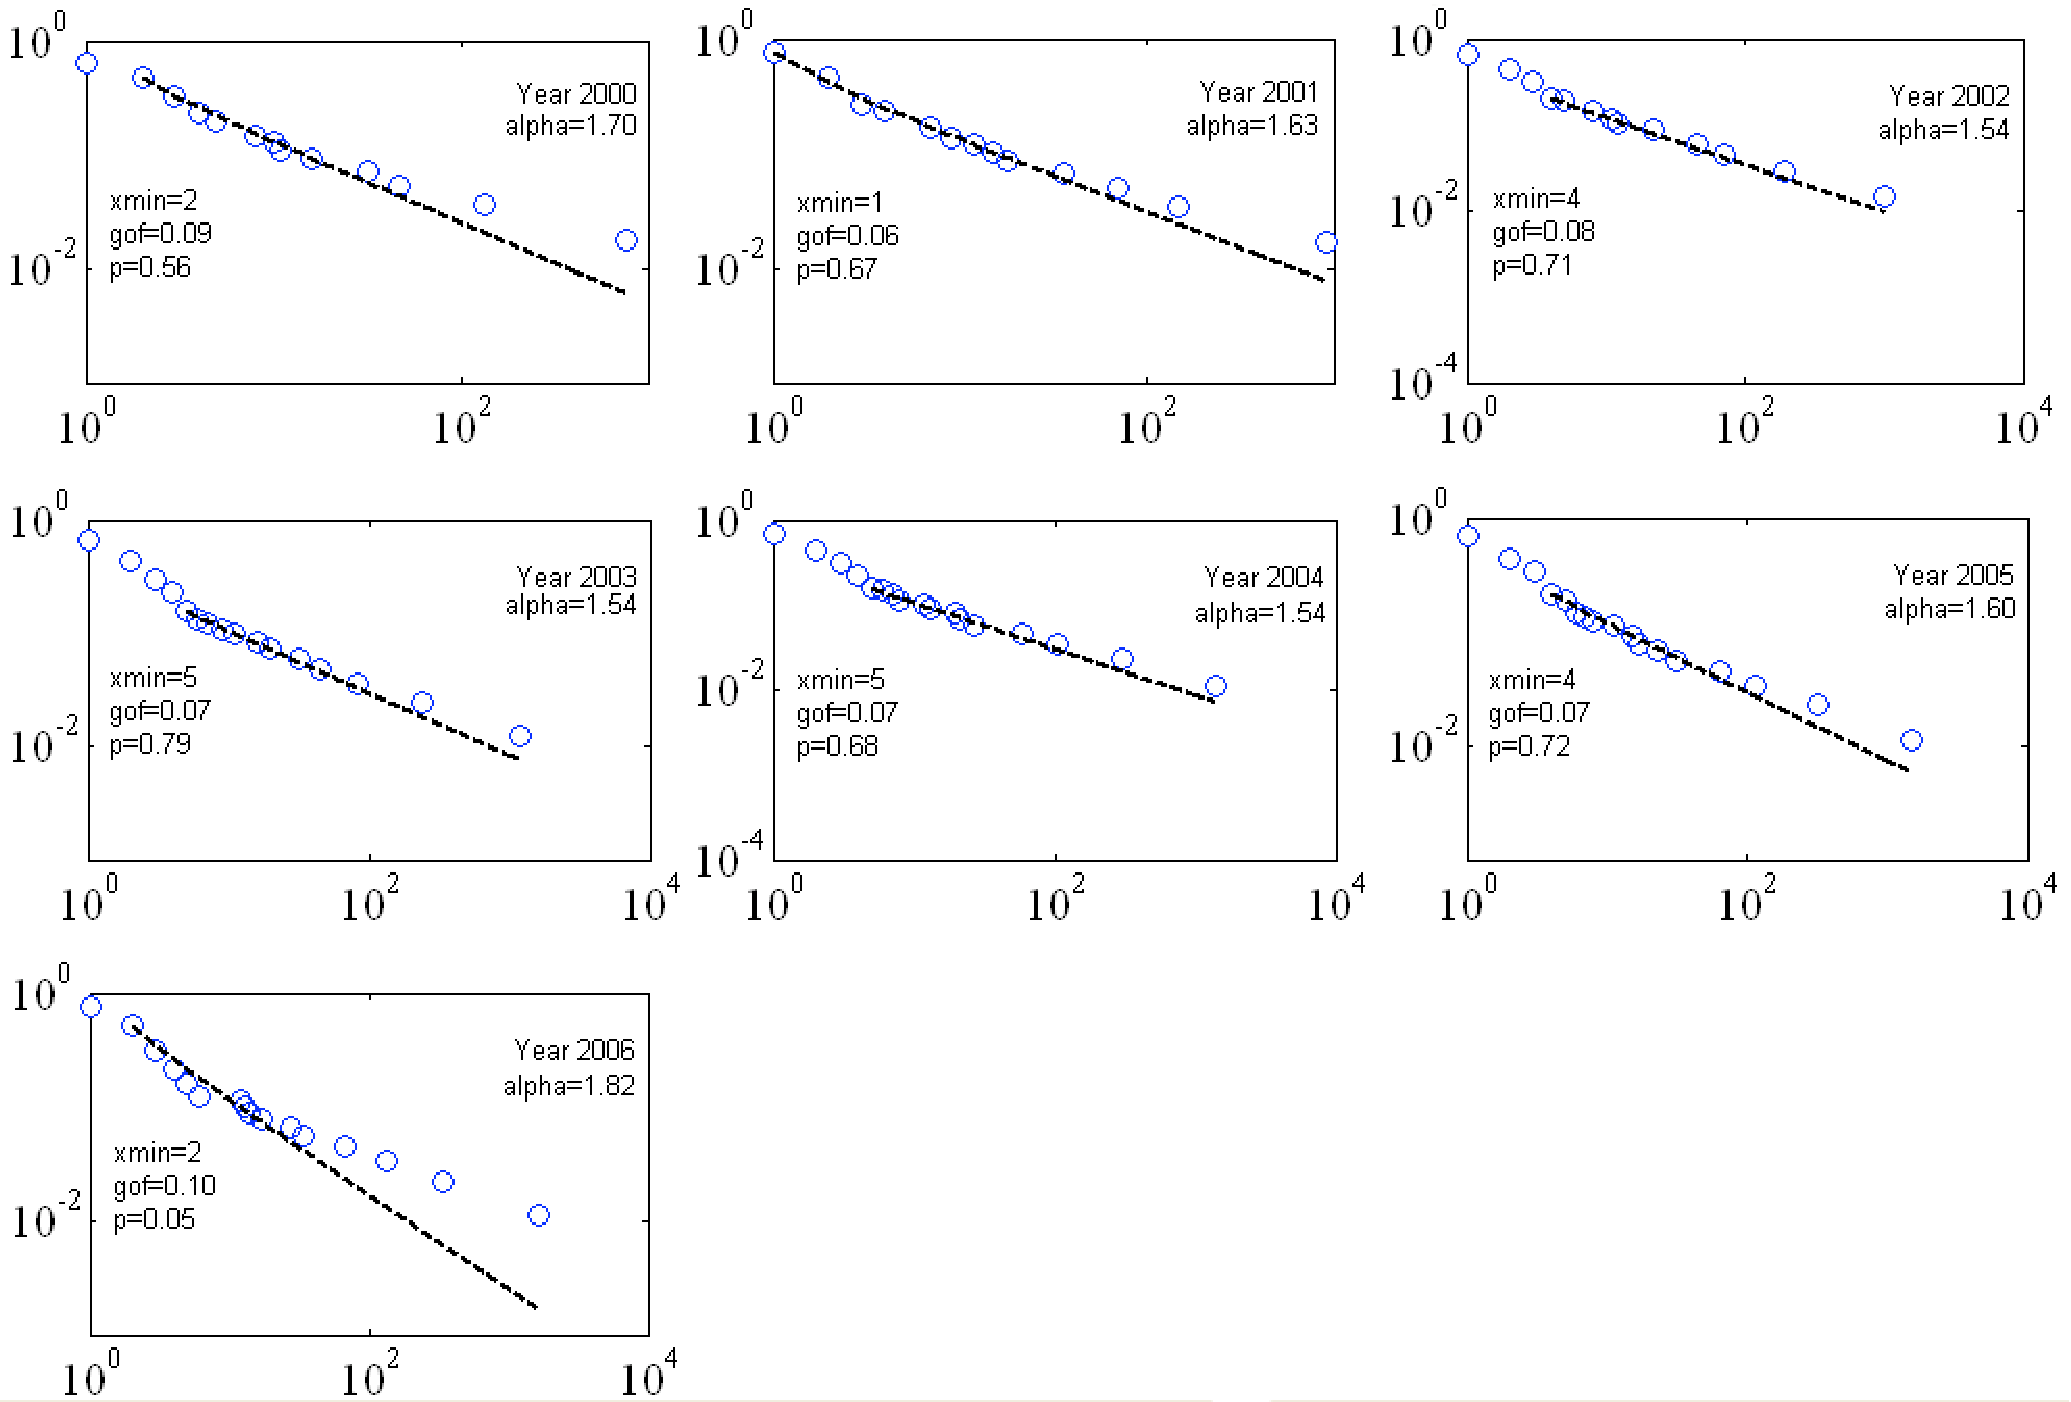
\includegraphics[width=\textwidth]{images/clausetcumulative}
\caption{Power law investigations. A power law is fitted to each years data and various statistics calculated: the exponent alpha, xmin, goodness-of-fit (gof) and p-value.}
\label{fig:clausetcumulative}
\end{figure*}


\begin{table}[htb]
\resizebox{\columnwidth}{!}{
\centering
\begin{tabular}{|p{48pt}|l|l|l|l|l|l|l|l|l|}
\hline
\multicolumn{1}{|c|}{Gang} & 1999 & 2000 & 2001 & 2002 & 2003 & 2004 & 2005 & 2006 & 2007 \\
\hline
\multicolumn{1}{|c|}{A} & \textbf{2.65} &  1.47 & 1.00 & \textbf{1.91} & 1.07 & 0.10 & 0.94 & 0.77 & 0.74 \\
\hline
\multicolumn{1}{|c|}{B} & \textbf{2.95}& 1.44& \textbf{3.64}& \textbf{1.88}& 1.36& 0.09& 0.97& 0.63& 0.51 \\
\hline
\multicolumn{1}{|c|}{C} & 0.27& 0.24& 0.17& 0.32& 0.38& 0.02& 0.46& 0.36& 0.32 \\
\hline
\multicolumn{1}{|c|}{D} & 1.26& 0.76& 0.56& 0.69& 1.14& 0.03& 1.21& 0.81& 0.65 \\
\hline
\end{tabular}}
\caption{Power law exponents for gangs, against years. Significant results are shown in bold-face.}
\label{tab:clausetgangyears}
\end{table}

Based on these experiments we are therefore unable to comment whether
the networks possessing scale-free characteristics, however we can
conclude that we have small-world networks, since consistently there
are larger clustering coefficients and shorter path lengths compared
to a random network with same number of gang members. This means two
things for our system:

\begin{itemize}
\item The smaller path length means that the criminal activity
(contagion) spreads more easily in this network than in a random
network.
\item Larger clustering coefficient means that contacts of contacts
are treated as contacts as well.
\end{itemize}


\subsection{Emergence of gangs}\label{sec:emergence}
We might see changes in the path length and clustering
coefficients from 2000 to 2005, indications of how the gangs have
become more closely knit or are splitting apart. By examining annual
links for 2001 and 2004, we might predict that the cumulative links
decrease and the annual links increase, just before/as a gang forms,
then both values increase afterwards as everyone becomes linked
together. This is not the case, and neither are we able to see any
meaningful behaviour in these data.

Figures~\ref{fig:all} and~\ref{fig:gangscc1years} show the clustering
coefficients for each gang and against years, and is also a pictorial
view of the new links per year. In Table~\ref{fig:gangscc1years} the
CC value of each gang dips at 2004. What this may indicate is
clustering due to non-gang members (from
Figure~\ref{fig:2002core_labelled}, offenders who are connected to
gang members: \emph{a*}, \emph{b*}, \emph{bc*} and \emph{ab*}) and
less clustering that previous years between members of gangs
themselves. There is also a significant peak in clustering during 2001
for Gang B, whereas all other gangs suffer a decrease in clustering.


\begin{figure*}[!ht]
\centering
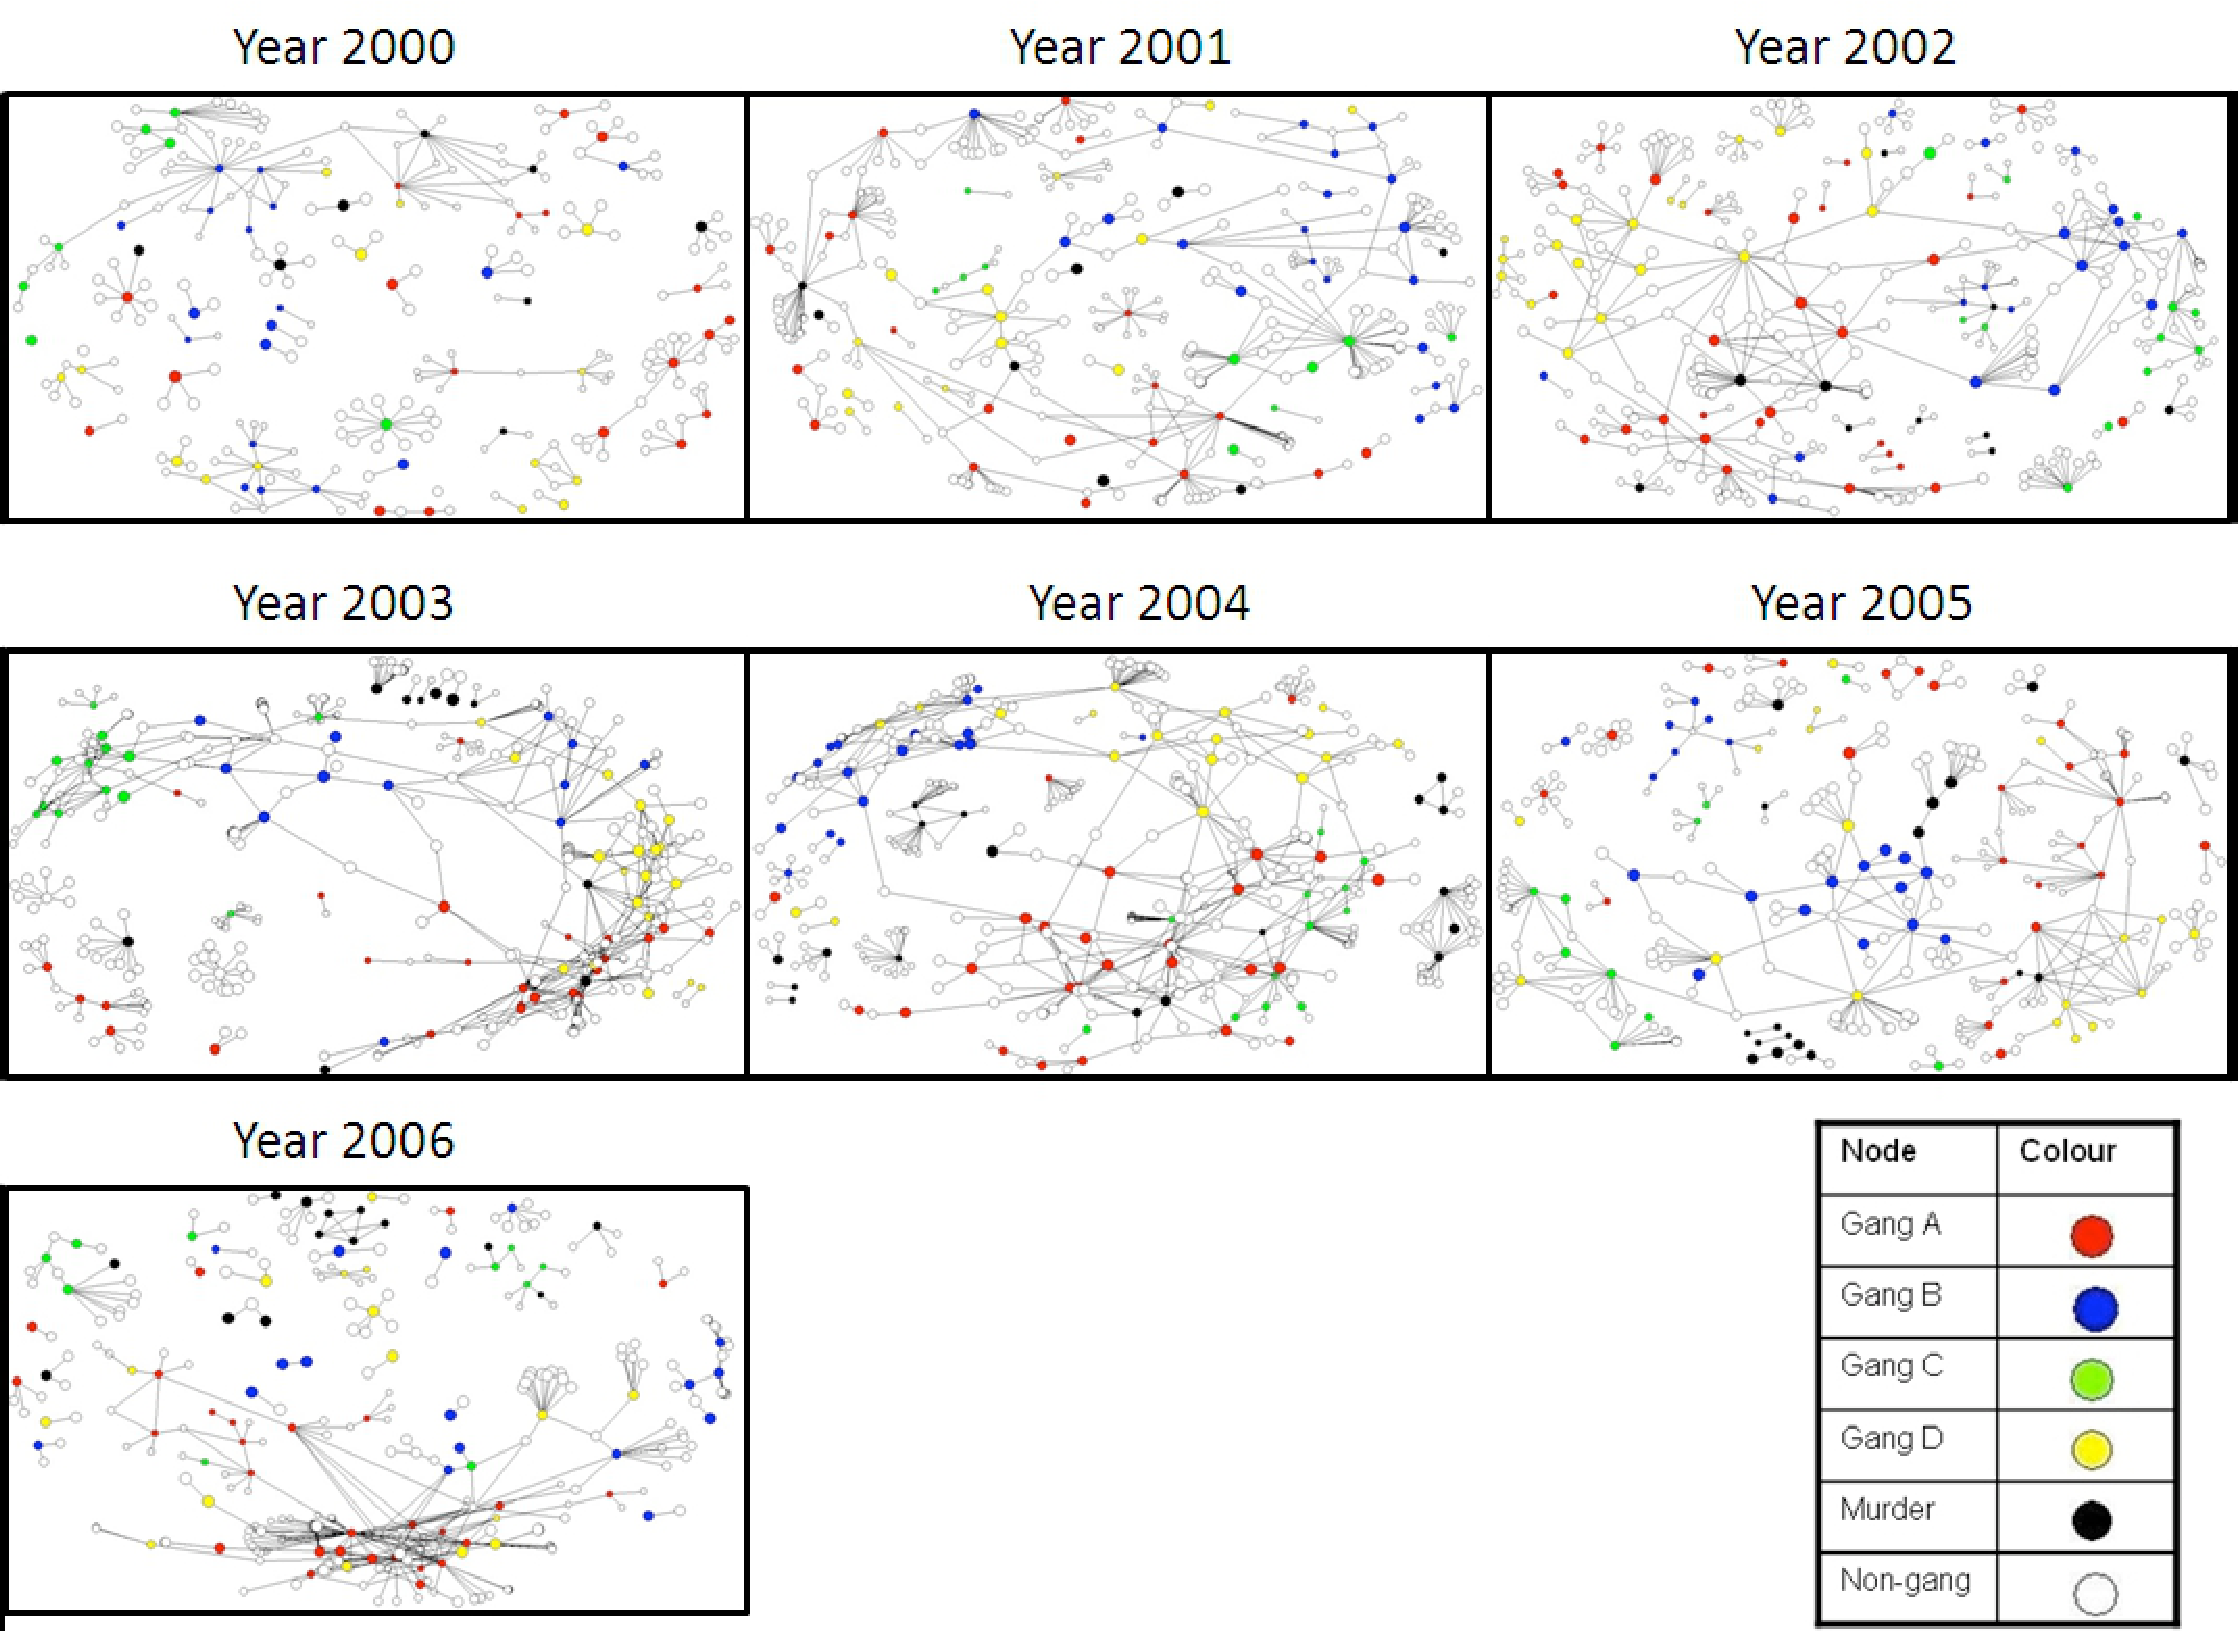
\includegraphics[width=\textwidth]{images/all}
\caption{Annual links formation. Only nodes directly connected to a gang member are included. The network measures for each of these networks can be found in Table~\ref{tab:networkmeasuresgang}.}
\label{fig:all}
\end{figure*}


\begin{figure}[htb]
\centering
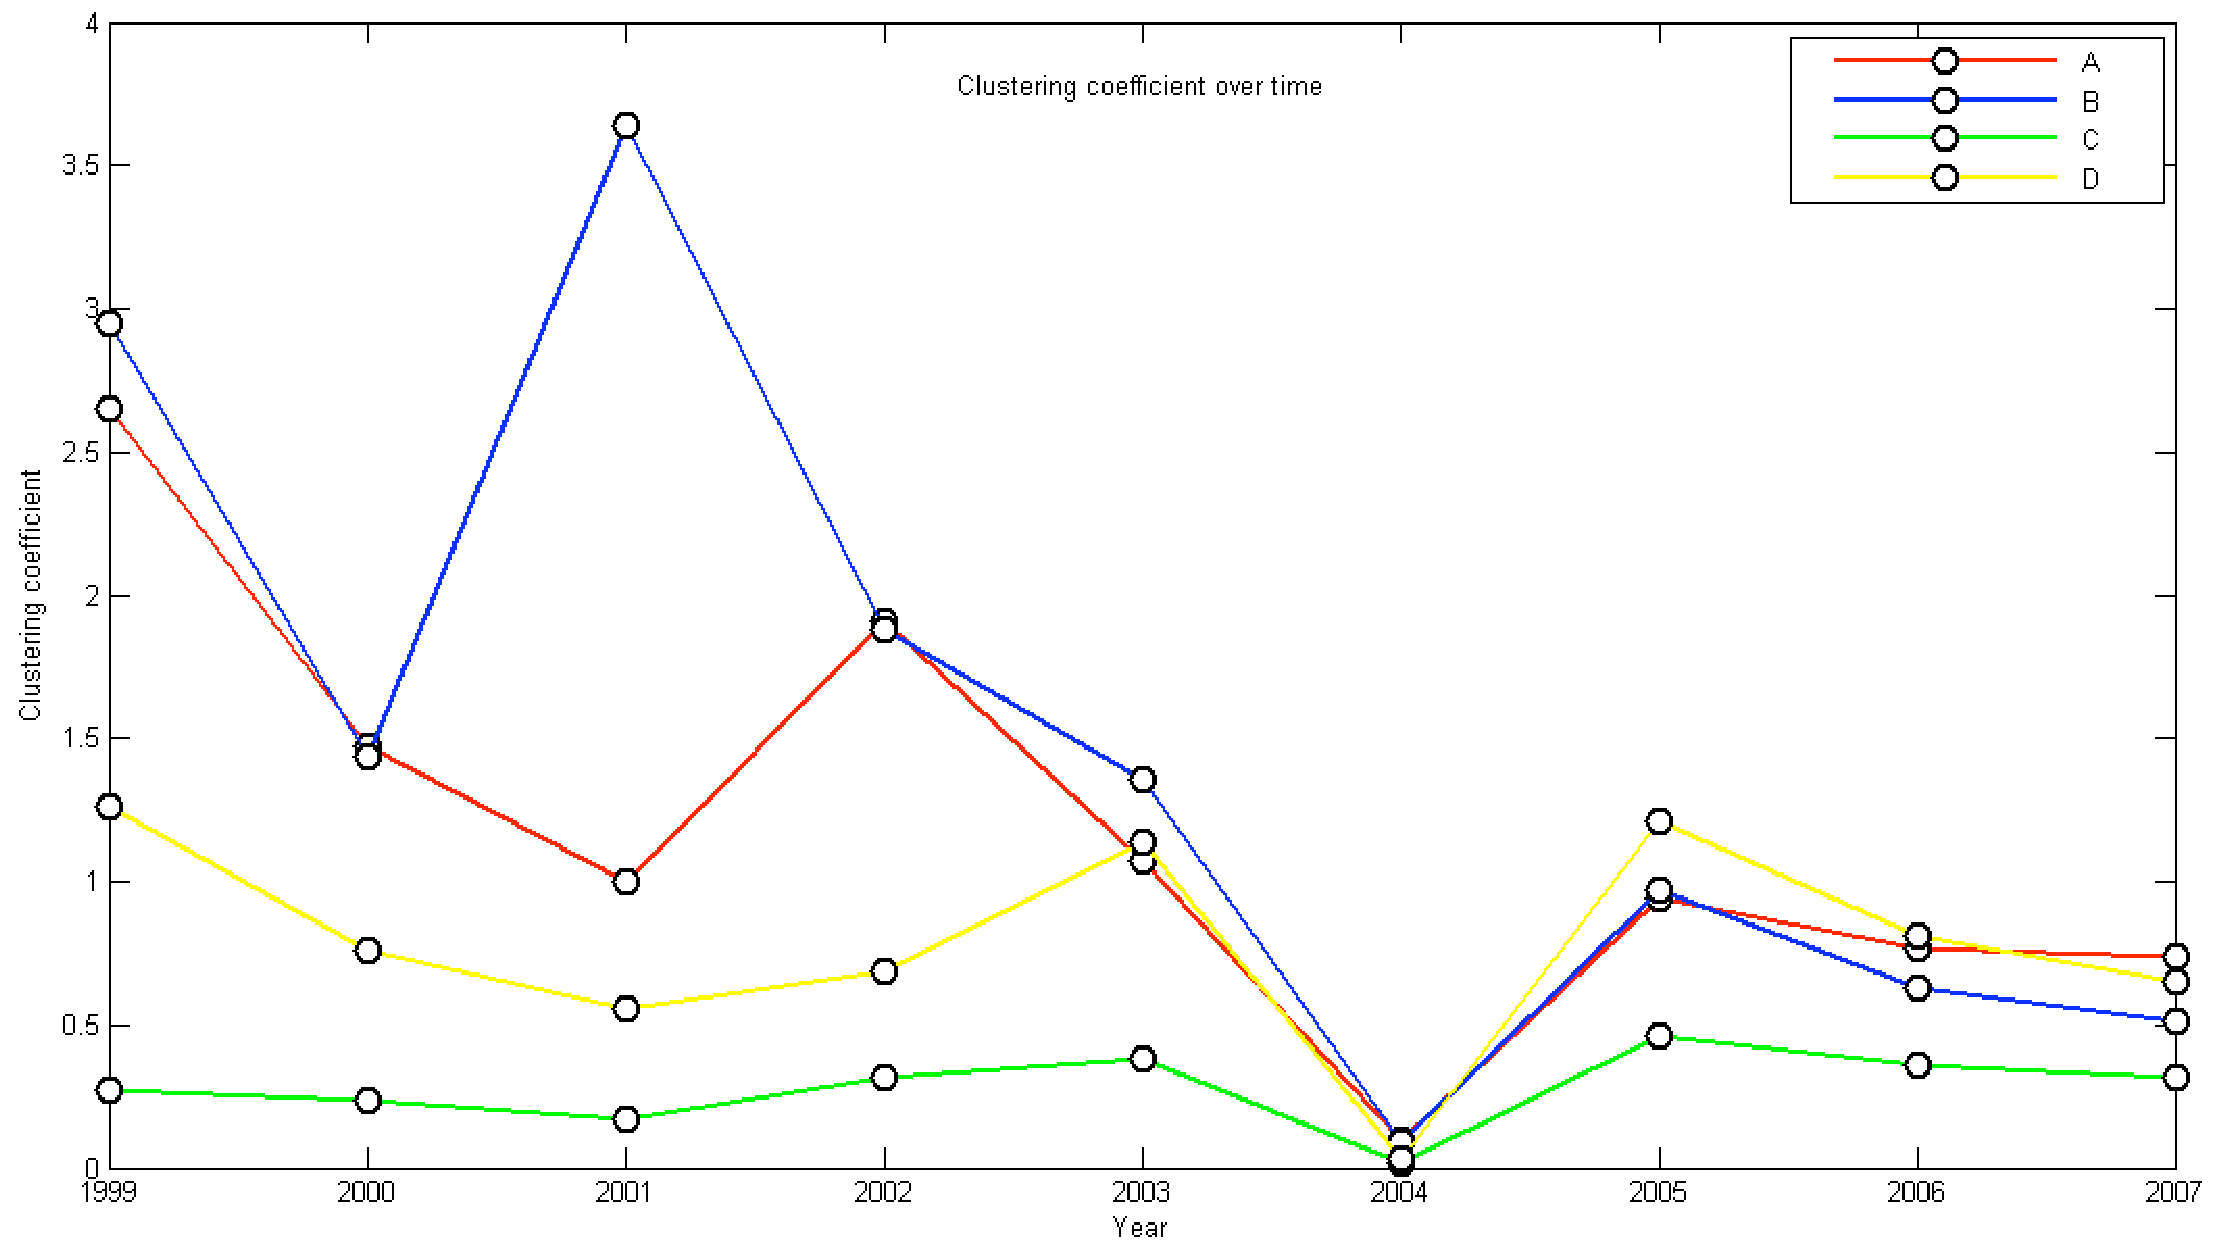
\includegraphics[width=\columnwidth]{images/gangscc1years}
\caption{Per year clustering coefficients for each gang. Gang C was formed in 2001, Gang D in 2004.} 
\label{fig:gangscc1years}
\end{figure}


\section{Discussion}\label{sec:discussion}
The model of two rival sets of gangs is potentially a
misrepresentation of the much more complex sets of smaller cliques and
fluid changes within the larger gang structures. However, the four
gangs discussed do exist, and are the main gangs; what is not possible
is a high degree of exactitude.

\subsection{External and internal factors}
It is difficult to determine through the gathered data what is
happening in the networks. We have little recorded evidence of gang
formation, even knowing when these events `allegedly' occurred,
similarly with the alleged `melt-down' following the death of
prominent gang leader Raymond Pitt in 1995~\cite{Walsh2005}. The links
are based upon observations by police officers -- do we expect that
these complex social situations can be reflected in the reported
links? Can we detect these events, and did they really happen as they
have been passed down to us? We are in the difficult situation of
using intelligence instead of concrete facts, and this intelligence is
often a poor reflection of what is happening in the chaotic social
world of gang culture.

We require a much better analysis of link types, developed a model
where individuals learn about crime opportunities by interacting with
other peers; for instance whether weak ties play an important role in
explaining criminal activities~\cite{PatacchiniZenou2008}, especially
gang homicide~\cite{papachristos:2009}.

The theoretical predictions of the model are confirmed by the
empirical analysis since they find that weak ties, as measured by
friends of friends, have a positive impact on criminal activities.

Furthermore, for 2001 and 2004, it would be interesting to examine the
kinds of links within each gang which split apart.

\subsection{Covert links}
Data collection is very partial and certainly biased, since not every
actor is exposed to an equal extent and therefore some of those
observed (perhaps the `usual suspects') contribute far more to the
dataset than others. Our earlier observation of a decrease in
clustering as the network temporarily fragments, before an increase in
clustering as everyone becomes linked together (as commented upon in
Section~\ref{sec:emergence}) finds equal explanation through the
police having intelligence on the formation of a new gang and actively
seeking observations on this event.

\section{Conclusions}\label{sec:conclusion}
The work presented in this paper contains our initial findings about
the offender/gang networks in Manchester in the UK, using network
analysis. The uses of this technology in an operational context are
significant. Even using the networks merely as visual representations
of otherwise cognitively unmanageable data contained in spreadsheets
and databases is operationally very useful, for knowledge sharing and
training, and identifying key offenders. When further pre-processing
is carried out, and the quality of the data collection process is
improved, there will be sigificant future work available with this
dataset.

The police crime recording database is routinely gathered and
available for analysis. The additional databases of histories and
associates of gang offenders are routinely gathered by the UK's
National Crime
Agency~\footnote{\url{http://www.nationalcrimeagency.gov.uk/}}, who
investigate gang and gun-related crimes. These data sources are
potential rich sources of information for computer science
technologies to deliver crime prevention and detection decision
support systems.

Criminal behaviour (modus operandi and offence profiling) is to be
incorporated into social network analysis.  This approach uses
retrospective methodologies, appropriate given the time scale and the
pilot nature of most work. Future work must be given the resources to
adopt prospective methods in order to increase the validity of
decisions concerning their contribution.


\section*{Acknowledgments}
We acknowledge the UK's Engineering \& Physical Sciences Research
Council (EPSRC) Sandpit on Gun Crime (September 2005, Warwickshire,
UK), funded by the IDEAS Factory; and the assistance of Xcalibre, the Greater
Manchester Police's specialist gang crime task force.

% trigger a \newpage just before the given reference
% number - used to balance the columns on the last page
% adjust value as needed - may need to be readjusted if
% the document is modified later
%\IEEEtriggeratref{37}
% The "triggered" command can be changed if desired:
%\IEEEtriggercmd{\enlargethispage{-5in}}

% BibTeX users
\bibliographystyle{IEEEtran}      % basic style, author-year citations
\bibliography{asonam2014}   % name your BibTeX data base

\end{document}
% end of file template.tex

